\section{Anhang}

\subsection{Massenträgheitsmomente}\label{Massenträgheitsmomente}

\begin{ctabular}{| c | c |}
  \hline
  \textbf{Zylinder / Scheibe}                                                 & \textbf{Hohlzylinder}                                                     \\
  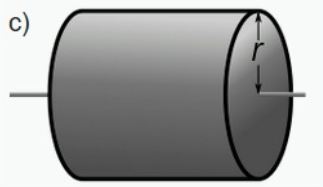
\includegraphics[width=0.35\columnwidth]{images/J_zylinder.png}             & 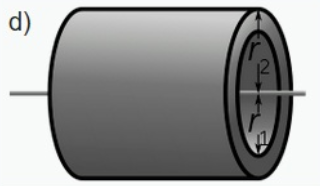
\includegraphics[width=0.35\columnwidth]{images/J_hohlzylinder.png}       \\
  $J = \frac{1}{2} m r^2$                                                     & $J = m \, \frac{r_1^2 + r_2^2}{2}$                                        \\
  \hline
  \textbf{Dünner Stab (Mitte)}                                                & \textbf{Dünner Stab (Ende)}                                               \\
  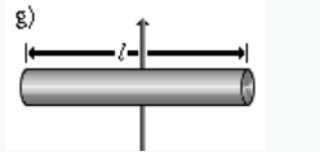
\includegraphics[width=0.35\columnwidth]{images/J_duenner_stab_mitte.png}   & 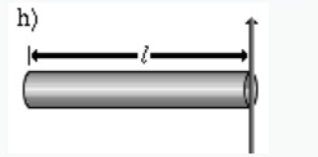
\includegraphics[width=0.35\columnwidth]{images/J_duenner_stab_ende.png}  \\
  $J = \frac{1}{12} m l^2$                                                    & $J = \frac{1}{3} m l^2$                                                   \\
  \hline
  \textbf{Kugel}                                                              & \textbf{Massenpunkt}                                                      \\
  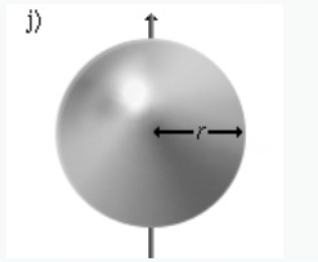
\includegraphics[width=0.35\columnwidth]{images/J_kugel.png}                & 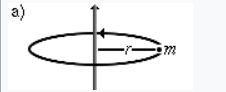
\includegraphics[width=0.35\columnwidth]{images/J_massepunkt.png}         \\
  $J = \frac{2}{5} m r^2$                                                     & $J = m r^2$                                                               \\
  \hline
\end{ctabular}

\subsection{Messunsicherheit \& geltende Stellen}

\[
  \Delta y = \sqrt{\sum_{i} \left( \frac{\partial y}{\partial x_i} \right)^2 \cdot \Delta x_i^2}
\]

\begin{ctabular}{| c | c | c | c |}
  \hline
  \textbf{Unsicherheit} & \textbf{Führende Ziffer} & \textbf{Gerundete Unsicherheit} & \textbf{Nachkommastellen} \\
  \hline
  0.30 & 3 & 0.3 & 1 \\
  0.25 & 2 & 0.25 & 2 \\
  0.002 & 2 & 0.0020 & 4 \\
  0.005 & 5 & 0.005 & 3 \\
  \hline
\end{ctabular}

\begin{itemize}
  \item Unsicherheit: 1--2 geltende Stellen (zwei nur bei führender 1 oder 2).
  \item Messwert: letzte Ziffer auf derselben Dezimalstelle wie die letzte Ziffer der Unsicherheit.
\end{itemize}

\subsection{Trigonometrie}

\begingroup
\renewcommand{\arraystretch}{2}
\setlength{\tabcolsep}{0mm}
\scalebox{0.33}{
  \Huge
  \begin{tabularx}{3\columnwidth}{rp{1mm}V{3}*{17}{C}}
    \rowcolor{subsectioncolor!30}$\bm{\alpha}$\phantom{${}^{\circ}$} && $0$ & $\dfrac{\pi}{6\mathstrut}$ & $\dfrac{\pi}{4}$ & $\dfrac{\pi}{3}$ & $\dfrac{\pi}{2}$ & $\dfrac{2\pi}{3}$ & $\dfrac{3\pi}{4}$ & $\dfrac{5\pi}{6}$ & $\pi$ & $\dfrac{7\pi}{6}$ & $\dfrac{5\pi}{4}$ & $\dfrac{4\pi}{3}$ & $\dfrac{3\pi}{2}$ & $\dfrac{5\pi}{3}$ & $\dfrac{7\pi}{4}$ & $\dfrac{11\pi}{6}$ & $2\pi$ \\\hline
    \rowcolor{subsectioncolor!30}$\bm{\alpha^\circ}$ && \phantom{${}^\circ$}$0^\circ$ & $30^\circ$ & $45^\circ$ & $60^\circ$ & $90^\circ$ & $120^\circ$ & $135^\circ$ & $150^\circ$ & $180^\circ$ & $210^\circ$ & $225^\circ$ & $240^\circ$ & $270^\circ$ & $300^\circ$ & $315^\circ$ & $330^\circ$ & $360^\circ$ \\\hline
    $\bm{\sin(\alpha)}$ && $0$ & $\dfrac{1}{2\mathstrut}$ & $\dfrac{\sqrt{2}}{2}$ & $\dfrac{\sqrt{3}}{2}$ & $1$ & $\dfrac{\sqrt{3}}{2}$ & $\dfrac{\sqrt{2}}{2}$ & $\dfrac{1}{2}$ & $0$ & $-\dfrac{1}{2}$ & $-\dfrac{\sqrt{2}}{2}$ & $-\dfrac{\sqrt{3}}{2}$ & $-1$ & $-\dfrac{\sqrt{3}}{2}$ & $-\dfrac{\sqrt{2}}{2}$ & $-\dfrac{1}{2}$ & $0$ \\\hline
    $\bm{\cos(\alpha)}$ && $1$ & $\dfrac{\sqrt{3}}{2\mathstrut}$ & $\dfrac{\sqrt{2}}{2}$ & $\dfrac{1}{2}$ & $0$ & $-\dfrac{1}{2}$ & $-\dfrac{\sqrt{2}}{2}$ & $-\dfrac{\sqrt{3}}{2}$ & $-1$ & $-\dfrac{\sqrt{3}}{2}$ & $-\dfrac{\sqrt{2}}{2}$ & $-\dfrac{1}{2}$ & $0$ & $\dfrac{1}{2}$ & $\dfrac{\sqrt{2}}{2}$ & $\dfrac{\sqrt{3}}{2}$ & $1$ \\\hline
    $\bm{\tan(\alpha)}$ && $0$ & $\dfrac{\sqrt{3}}{3\mathstrut}$ & $1$ & $\sqrt{3}$ & $\pm\infty$ & $-\sqrt{3}$ & $-1$ & $-\dfrac{\sqrt{3}}{3}$ & $0$ & $\dfrac{\sqrt{3}}{3}$ & $1$ & $\sqrt{3}$ & $\pm\infty$ & $-\sqrt{3}$ & $-1$ & $-\dfrac{\sqrt{3}}{3}$ & $0$ \\\hline
    $\bm{\cot(\alpha)}$ && $\pm\infty$ & $\sqrt{3}$ & $1$ & $\dfrac{\sqrt{3}}{3\mathstrut}$ & $0$ & $-\dfrac{\sqrt{3}}{3}$ & $-1$ & $-\sqrt{3}$ & $\pm\infty$ & $\sqrt{3}$ & $1$ & $\dfrac{\sqrt{3}}{3}$ & $0$ & $-\dfrac{\sqrt{3}}{3}$ & $-1$ & $-\sqrt{3}$ & $\pm\infty$ \\
\end{tabularx}}
\endgroup

\subsubsection{Beziehungen zwischen $\bm{\sin(x)}$ und $\bm{\cos(x)$}}

\begin{tabular}{lll}
  $\sin(-a) = -\sin(a)$   & $\sin(\pi - a) = \sin(a)$     & $\sin(\pi + a) = -\sin(a)$ \\
  $\cos(-a) = \cos(a)$    & $\cos(\pi - a) = - \cos(a)$   & $\cos(\pi + a) = - \cos(a)$ \\
  \\
\end{tabular}

\begin{tabular}{ll}
  $\sin(\frac{\pi}{2} - a) = \sin(\frac{\pi}{2} + a) = \cos(a)$ & $\cos(\frac{\pi}{2} - a) = - \cos(\frac{\pi}{2} + a) = \sin(a)$
\end{tabular}

\subsubsection{Additionstheoreme}

\begin{tabular}{ll}
  $\sin(a \pm b) = \sin(a) \cdot \cos(b) \pm \cos(a) \cdot \sin(b)$   & $\tan(a \pm b) = \frac{\tan(a) \pm \tan(b)}{1 \mp \tan(a) \cdot \tan(b)}$\\
  $\cos(a \pm b) = \cos(a) \cdot \cos(b) \mp \sin(a) \cdot \sin(b)$   &
\end{tabular}

\subsubsection{Summen und Differenzen}

\renewcommand{\arraystretch}{1.5}
\begin{tabular}{ll@{}}
  $\sin(a) + \sin(b) = 2 \cdot \sin \big( \frac{a+b}{2} \big) \cdot \cos \big( \frac{a-b}{2} \big)$ &
  $\cos(a) + \cos(b) = 2 \cdot \cos \big( \frac{a+b}{2} \big) \cdot \cos \big( \frac{a-b}{2} \big)$ \\
  $\sin(a) - \sin(b) = 2 \cdot \sin \big( \frac{a-b}{2} \big) \cdot \cos \big( \frac{a+b}{2} \big)$ &
  $\cos(a) - \cos(b) = -2 \cdot \sin \big( \frac{a+b}{2} \big) \cdot \sin \big( \frac{a-b}{2} \big)$ \\
  $\tan(a) \pm \tan(b) = \frac{\sin(a \pm b)}{\cos(a) \cdot \cos(b)}$
\end{tabular}
\renewcommand{\arraystretch}{1}

\subsubsection{Produkte}

$\sin(a) \cdot \sin(b) = \frac{1}{2} \big( \cos(a-b) - \cos(a+b) \big) $ \\
$\cos(a) \cdot \cos(b) = \frac{1}{2} \big( \cos(a-b) + \cos(a+b) \big) $ \\
$\sin(a) \cdot \cos(b) = \frac{1}{2} \big( \sin(a-b) + \sin(a+b) \big) $


\subsubsection{Winkelvielfache und Halbwinkel}

\renewcommand{\arraystretch}{1.3}
\begin{tabular}{ll}
  $\sin(2a) = 2 \, \sin(a) \cdot \cos(a)$                         & $\cos(2a) = \cos^2(a) - \sin^2(a)$                                \\
  $\sin(3a) = 3 \, \sin(a) -4 \, \sin^3(a)$                       & $\cos(3a) = 4 \, \cos^3(a) -3 \, \cos(a)$                         \\
  $\sin \big( \frac{a}{2} \big) = \sqrt{\frac{1}{2}(1-\cos(a))} $ & $\cos \big( \frac{a}{2} \big) = \sqrt{\frac{1}{2}(1+\cos(a))} $
\end{tabular}

\subsubsection{Potenzen}

\renewcommand{\arraystretch}{1.5}
\begin{tabular}{ll}
  $\sin^2(a) = \frac{1^{\mathstrut}}{2}(1-\cos(2a))$               & $\cos^2(a) = \frac{1}{2}(1+\cos(2a))$                \\
  $\sin^3(a) = \frac{1^{\mathstrut}}{4}(3\, \sin(a) - \sin(3a))$   & $\cos^3(a) = \frac{1}{4}(\cos(3a) + 3 \, \cos(a))$
\end{tabular}
\renewcommand{\arraystretch}{1}
